%%%%%%%%%%%
% Preface %
%%%%%%%%%%%

This document describes {\sc Mnemosyne}, a prototype CAD tool under\footnote{The development of {\sc Mnemosyne} started within the System-Level Design Group at Columbia
University: \url{http://www.sld.cs.columbia.edu}} for the
optimization of the {\bf Private Local Memory} of specialized
accelerators.
%%
More specifically, we target loosely-coupled accelerators and other hardware components that are
organized as shown in Fig.~\ref{fig:accelerator}.

\begin{figure}[h!]
  \centering
  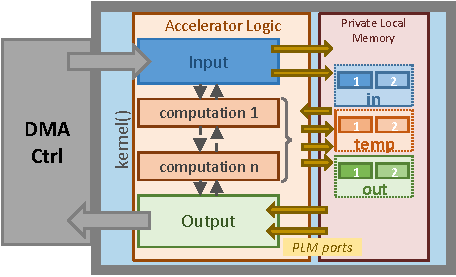
\includegraphics[width=0.5\columnwidth]{fig/accelerator.pdf}
  \caption{Organization of our loosely-coupled accelerators.}\label{fig:accelerator}
\end{figure}

Each accelerator is composed of two parts: the accelerator logic and
the private local memory. The {\bf Accelerator Logic} is composed of
multiple concurrent hardware blocks to manage the data transfers
(e.g. {\em Input} and {\em Output}) and perform the actual computation
(e.g. {\em Computation$_k$}). The {\bf Private Local Memory} (PLM)
locally stores the data structures used by the accelerator to perform
the computation so that they can be accessed with fixed latency by the
accelerator logic. For doing this, it is organized in multiple banks
implemented with area-efficient memory Intellectual Property (IP)
blocks to offer the possibility of multiple concurrent accesses
through different {\em PLM ports}. Each PLM port is connected to a
{\em process interface} in the accelerator logic, which generates the
corresponding memory request.

The rest of this document is organized as follows:
\begin{itemize}
\item Chapter~\ref{ch:methodology} describes the methodology
  implemented by {\sc Mnemosyne};
\item Chapter~\ref{ch:tool} presents the tool, including information
  for installation and configuration;
\item Chapter~\ref{ch:mem_interface} describes the interface of the
  memory IP blocks which is assumed by {\sc Mnemosyne};
\item Chapter~\ref{ch:proc_interface} describes the PLM interface
  generated by {\sc Mnemosyne} to be connected to the rest of the
  accelerator logic.
\end{itemize}

